\chapter{Modélisation d'un drone convertible : DarkO}
\minitoc

\section{Modèle du drone DarkO}
\label{sec:model}
DarkO est un drone conçu et développé à l'École Nationale de l'Aviation Civile (ENAC) de Toulouse (France), est un exemple clair de drone convertible avec une architecture dite \textit{tail-sitter}.
DarkO est assemblé à partir de plusieurs pièces d'Onyx imprimées en 3D (un matériau très robuste composé de fibres de carbone omnidirectionnelles). Toutes les pièces sont emboîtées sur un seul axe, de sorte que le drone puisse facilement être démonté pour remplacer des pièces ou accéder à l'électronique embarquée. 

L'autopilote embarqué est une carte Apogee~\footnote{\url{https://wiki.paparazziuav.org/wiki/Apogee/v1.00}} fabriquée à l'ENAC, voir Fig. \ref{fig:apogee}. 


\begin{figure}[ht]
    \centering
        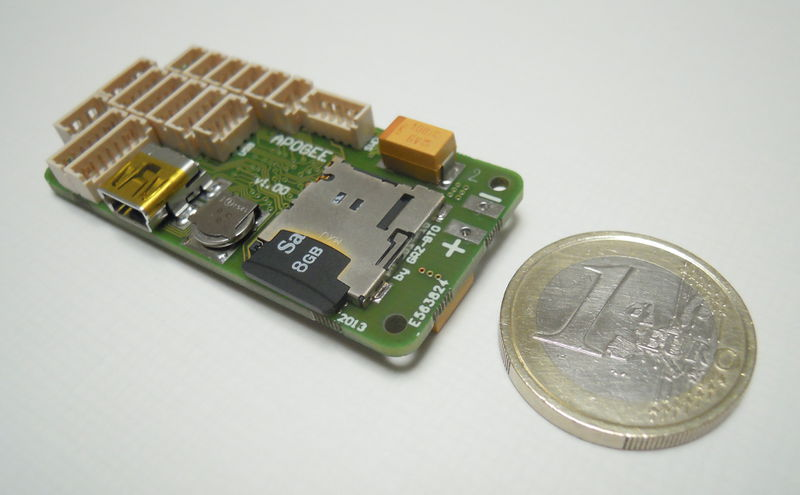
\includegraphics[width=0.8\columnwidth]{figures/800px-Apogee_v100_top_1E.jpeg}
        \caption{Vue de dessus d'un autopilote Apogee v1.00.}
        \label{fig:apogee}
\end{figure}

L'autopilote offre la possibilité d'enregistrer les données de bord sur une carte mémoire SD, à la fréquence de contrôle de 500 Hz, ce qui permet un post-traitement efficace des données acquises. Le protocole de communication utilisé entre l'autopilote et les contrôleurs électroniques de vitesse (ESC) est le Dshot 600. Les ESC sont des AIKON AK32 35A \todo{trouver un synonyme} flasher avec un firmware AM32. La communication sol-bord est réalisée via un canal bidirectionnel basé sur des modules XBee-PRO S1.

\begin{figure}[ht]
    \centering
    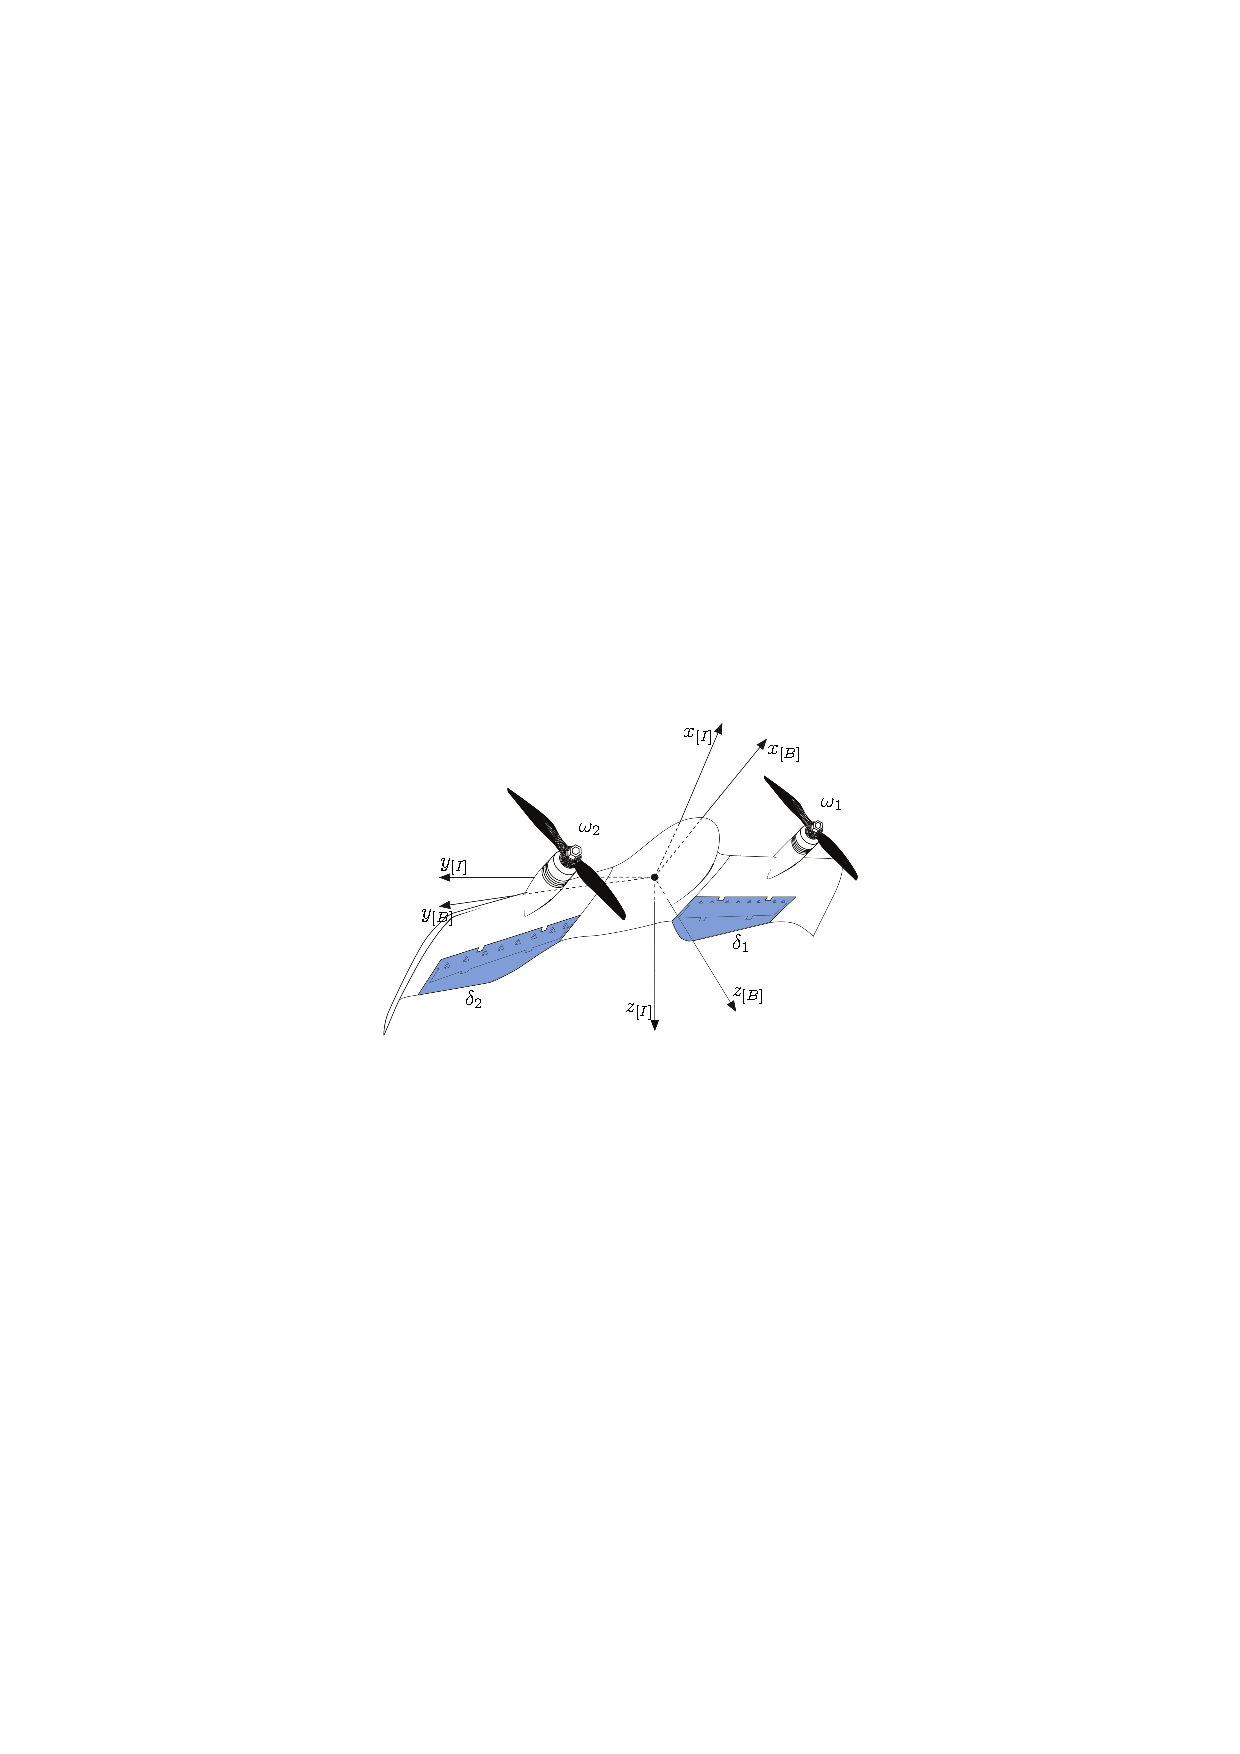
\includegraphics[width=1\columnwidth]{figures/darko.pdf}
    \caption{Repère de référence de DarkO avec une représentation schématique des actionneurs.}
    \label{fig:darko2}
\end{figure}

Les actionneurs de DarkO peuvent être décomposé en deux catégories. La première est composée de deux hélices (T-Motor T5147) placées symétriquement à l'avant de l'aile (illustrées en \textbf{noir} dans la Fig. \ref{fig:darko2}) alimentées par deux moteurs électriques (T-Motor F30 2300kv) générant une traction selon l'axe $x_{b}$. La seconde catégorire est relative aux actionneurs aérodynamiques ainsi le drone possède deux élevons, placés à l'arrière de l'aile (illustrés en \textcolor{cyan}{bleu} dans la Fig. \ref{fig:darko2}), agissant en tant que surfaces de contrôle. Les élevons génèrent des forces et des moments en modifiant leurs incidences relativement au flux d'air dans lequel ils sont placé. Ce flux d'air peut être généré par le vent relatif (liée à la vitesse du drone), le vent extérieur, mais aussi par le souffle des hélices. Les élevons sont commandés par deux servomoteurs MKS DS65K. La figure \ref{fig:darko2} montre le modèle de DarkO, ainsi qu'un repère de référence inertiel NED (ou repère terrestre) ``$\text{i}$'' lié à la surface de la Terre, et un repère corps `$\text{b}$'' attaché au drone, avec $x_{\text{b}}$ correspondant à l'axe de roulis (l'axe des hélices dans le plan $z_{\text{b}} =0$), $y_{\text{b}}$ l'axe de tangage (la direction des ailes), $z_{\text{b}}$ l'axe de lacet. En utilisant la même notation que dans \cite{lustosa:hal-03035938}, le couple hélice/élévateur gauche et droit sont désignés par les indices $i=1$ (gauche) et $i=2$ (droite). La convention de signe sera définie comme positive pour les positions des élevons $\delta_{1}$, $\delta_{2}$ lorsqu'ils créent un moment à cabrer avec les hélices tournant dans des directions opposées avec des vitesses angulaires $\omega_{1} > 0$ et $\omega_{2} < 0$, respectivement.

\todo{traduire la table}
\begin{table}[ht]
    \centering
      \begin{tabular}{|l|c|c|}
        \hline
        \multicolumn{1}{|c|}{Parameter or coefficient} & Value & Units  \\
        \hline
        $m$ (drone mass)  & 0.519 & \SI{}{\kilogram} \\
        \hline
        $b$ (wingspan)  & 0.542 & \SI{}{\meter} \\
        \hline
        $c$ (aerodynamic cord)  & 0.13 & \SI{}{\meter} \\
        \hline
        $\boldsymbol{B}=\diag(b,c,b)$ & $\!\!\diag(0.542, 0.13, 0.542)$ \!\! & \SI{}{\meter}\\
        \hline
        $S$ (wing area) & 0.026936 & \SI{}{\square\meter}\\
        \hline
        $S_{\text{wet}}$ (wet area) & 0.0180 & \SI{}{\square\meter}\\
        \hline
        $S_{\text{p}}$ (propeller area) & 0.0127 & \SI{}{\square\meter}\\
        \hline
        % $J_{x}$ & 0.0070 & \SI{}{\kilogram\square\meter}\\
        % \hline
        $\boldsymbol{J}=\diag(J_{x},J_{y},J_{z})$ & \!\! $\diag(0.0072,0.0004,0.0086)$\!\! & \SI{}{\kilogram\square\meter}\\
        % \hline
        % $J_{z}$ & 0.0061 & \SI{}{\kilogram\square\meter}\\
      %   \hline
      %   $J_{p}$ & 5.1116e-6 & \SI{}{\kilogram\square\meter}\\
        \hline
        $k_{\text{f}}$ (propeller thrust) & 1.7800e-8 & \SI{}{\kilogram\meter}\\
        \hline
        $k_{\text{m}}$(propeller torque) & 2.1065e-10 & \SI{}{\kilogram\square\meter}\\
        \hline
        $p_{x}$ (propeller $x$ location) & 0.065 & \SI{}{\meter}\\
        \hline
        $p_{y}$ (propeller $y$ location) & 0.162 & \SI{}{\meter}\\
        \hline
        $a_{y}$ (lift $y$ position) & 0.1504 & \SI{}{\meter}\\
        \hline
        $\xi_{\text{f}}$ (elevons lift) & 0.2 & --\\
        \hline
        $\xi_{\text{m}}$ (elevons torque) & 1.4 & --\\
        \hline
        $\rho$ (air density) & 1.225 & \SI{}{\kilogram\per\cubic\meter}\\
        \hline
        $C_{\text{d}}$ (drag coefficient) & 0.1644 & --\\
        \hline
        $C_{y}$ (lateral coefficient) & 0 & --\\
        \hline
         $C_{\ell}$ (lift coefficient) & 5.4001 & --\\
        \hline
        $\Delta_{\text{r}}$ (UAV centering) & -0.0145 & \SI{}{\meter}\\
        \hline
      \end{tabular}
      \caption{\label{tab:pars} Identified numerical parameters of the DarkO model.}
\end{table}

\subsection{Modèle non-linéaire complet}

En exploitant la modélisation présentée dans \cite{lustosa:hal-03035938} et \cite{olszaneckibarth:hal-02542982}, un modèle précis de la dynamique de DarkO décrit la position $\boldsymbol{p} \in \real^3$ du centre de gravité et sa vitesse $\boldsymbol{v} = \dot{\boldsymbol{p}} \in \real^3$, en plus de son orientation, bien représentée par un quaternion $\boldsymbol{q} \in {\mathbb S}^3:=\{ \boldsymbol{q} \in \real^4 : |\boldsymbol{q}| = 1\}$ et de sa vitesse angulaire $\boldsymbol{\omega}_{\text{b}}$ représentée dans le repère du corps, qui satisfait $boldsymbol{\dot q} = \frac{1}{2}\boldsymbol{q} \otimes \smallmat{0 \\ \boldsymbol{\omega}_{{\text{b}}}}$, où $\otimes$ représente le produit de Hamilton (voir \cite{lustosa:hal-03035938,olszaneckibarth:hal-02542982} ou le tutoriel \cite{hamel_minhduc} pour plus de détails). En choisissant l'état global comme $\boldsymbol{x}:=(\boldsymbol{p},~ \boldsymbol{v},~ \boldsymbol{q},~ \boldsymbol{\omega}_{\text{b}})$, le modèle mathématique dérivé dans \cite{lustosa:hal-03035938}, dépendent d'un ensemble de paramètres énumérés dans le tableau \ref{tab:pars}, où nous indiquons également la valeur obtenue à partir d'une identification du système \cite{sansou:stage}. Le modèle dynamique peut être écrit comme ci-dessous :

\begin{subequations}\label{eq:dyna_orig}
    \begin{empheq}[left=\empheqlbrace]{alignat=2}
          % \boldsymbol{\dot p} & &= & \boldsymbol{v} \label{eq:dyna1}\\
          m\boldsymbol{\dot v} &&=& - m\boldsymbol{g} +  \boldsymbol{R}(\boldsymbol{q})\boldsymbol{F}_{\text{b}},\\
          \label{eq:dyna_orig_b}
          \boldsymbol{J} \boldsymbol{\dot \omega_{\text{b}}} &&= &  - \skewsym{\boldsymbol{\omega}_{\text{b}}}\boldsymbol{J}\boldsymbol{\omega}_{\text{b}} + \boldsymbol{M}_{\text{b}},
    \end{empheq}
  \end{subequations}
  où $\boldsymbol{g}:=\smallmat{0 & 0& 9.81}^\top$ désigne le vecteur de gravité, $m\in \real$ est la masse, $\boldsymbol{J}\in \real^{3\times 3}$ est le moment d'inertie diagonal (voir Tableau~\ref{tab:pars}) et en partitionnant le quaternion $\boldsymbol{q} \in {\mathbb S}^3$ comme $\boldsymbol{q} := \left[ \eta ~ \boldsymbol{\epsilon}^\top \right]^\top$, la matrice de rotation correspondante est $\boldsymbol{R}(\boldsymbol{q}) \in SO(3): = \{\boldsymbol{R}\in \real^{3\times 3}: \; \boldsymbol{R}^\top \boldsymbol{R} = \mathbb{I}_{3}, \det (\boldsymbol{R})=1\}$ est défini comme (voir \cite{hamel_minhduc})
\begin{align}
    \label{eq:matrix_rot}
    \boldsymbol{R}(\boldsymbol{q}) := \mathbb{I}_{3} +2\eta \skewsym{\boldsymbol{\epsilon}} + 2\skewsym{\boldsymbol{\epsilon}}^{2}.
\end{align}


D'après \cite{lustosa:hal-03035938} le vecteur de force et de moment $\boldsymbol{F}_{\text{b}}$ et $\boldsymbol{M}_{\text{b}}$ dans \eqref{eq:dyna_orig} dépendent  (i) de l'état du système $\boldsymbol{x}$, (ii) de la perturbation $\boldsymbol{w} \in \real^3$, représentant la vitesse du vent dans le référentiel inertiel, et (iii) de la commande des actionneurs (voir Figure~\ref{fig:darko2}), comprenant la vitesse de rotation des deux hélices $\omega_1, \omega_2 \in \real$ et la déflexion des élevons $\delta_1, \delta_2\in \real$.
Considérons d'abord l'effet des commandes des actionneurs. Chaque hélice génère une poussée $\boldsymbol{T}_i$ orienté dans la direction $x$ du repère corps et un moment $\boldsymbol{N}_i$ selon le même axe :
\begin{align}
\label{eq:thrust}
\boldsymbol{T}_{i} \!:=\! \begin{bmatrix} \tau_{i} \\ 0 \\ 0 \end{bmatrix} \!:=\!
\begin{bmatrix} k_{\text{f}}\omega_{i}^{2} \\ 0 \\ 0 \end{bmatrix}\! , \;
\boldsymbol{N}_{i} \!:=\! (-1)^{i}  \frac{k_{\text{m}} }{k_{\text{f}}}\boldsymbol{T}_{i}, \quad i=1,2 .
\end{align} 

La position de chaque élevon $\delta_i \in \real$ est assignée par un servomoteur qui impose un niveau d'efficacité (en termes de déviation du courant d'air) quantifié par deux matrices antisymétriques :
\begin{align}
\label{eq:elevons_efficiency}
    \boldsymbol{\Delta}^{\text{f}}_{i} \!:=\! \begin{bmatrix} 0 & 0 & \xi_{\text{f}}\delta_{i} \\ 0 & 0 & 0 \\ -\xi_{\text{f}}\delta_{i} & 0 & 0 \end{bmatrix}\! ,\;
    \boldsymbol{\Delta}^{\text{m}}_{i} \!:=\! \begin{bmatrix} 0 & 0 & \xi_{\text{m}}\delta_{i} \\ 0 & 0 & 0 \\ -\xi_{\text{m}}\delta_{i} & 0 & 0 \end{bmatrix} \!, 
\end{align}
$i=1,2$. Les paramètres constants $k_{\text{f}}$, $k_{\text{m}}$, $\xi_{\text{f}}$, $\xi_{\text{m}}$ apparaissant dans \eqref{eq:thrust} et \eqref{eq:elevons_efficiency} sont listés dans la Table~\ref{tab:pars}.\\
Avec les quantités ci-dessus, nous pouvons réarranger la dynamique donnée dans le tableau suivant \cite[eqns (97),~(98)]{lustosa:hal-03035938} (voir aussi \cite{sansou:stage}) et exprimer $\boldsymbol{F}_{\text{b}}$ et $\boldsymbol{M}_{\text{b}}$ dans \eqref{eq:dyna_orig} comme
%
\begin{align}
%\begin{split}
\nonumber
    \boldsymbol{F}_{\text{b}} :={}&  \boldsymbol{T}_{1} + \boldsymbol{T}_{2} + \frac{S_{\text{wet}}}{4S_{\text{p}}} \boldsymbol{\Phi}^{\text{(fv)}} \Big( (\boldsymbol{\Delta}^{\text{f}}_1 - \mathbb{I}_{3} ) \boldsymbol{T}_{1} + ( \boldsymbol{\Delta}^{\text{f}}_2 - \mathbb{I}_{3}) \boldsymbol{T}_{2}\Big) \\ 
     \label{eq:Fb}
    &+ \frac{1}{4} \rho S  \boldsymbol{\Phi}^{\text{(fv)}} \Big(\boldsymbol{\Delta}^{\text{f}}_1+ \boldsymbol{\Delta}^{\text{f}}_2 - 2 \mathbb{I}_{3} \Big) \lVert \boldsymbol{v_{\text{b}}} \rVert \boldsymbol{v_{\text{b}}}\\
    \nonumber
    &+ \frac{1}{4} \rho S \boldsymbol{\Phi}^{\text{(mv)}} \Big(\boldsymbol{\Delta}^{\text{f}}_1 + \boldsymbol{\Delta}^{\text{f}}_2 - 2\mathbb{I}_{3}\Big) \boldsymbol{B} \lVert \boldsymbol{v_{\text{b}}} \rVert  \boldsymbol{\omega}_{\text{b}}, 
%\end{split}
\end{align}
% 
\begin{align} 
\label{eq:Mb}
% \begin{split}
 \boldsymbol{M}_{\text{b}} :&=\boldsymbol{N}_{1} + \boldsymbol{N}_{2} + \skewsym{\smallm{p_x\\ p_y\\ 0}} \boldsymbol{T}_{1} + \skewsym{\smallm{p_x\\ - p_y\\ 0}} \boldsymbol{T}_{2}\\
    \nonumber
  &- \frac{S_{\text{wet}}}{4S_{\text{p}}} \bigg( \boldsymbol{B} \boldsymbol{\Phi}^{\text{(mv)}} (\boldsymbol{\Delta}^{\text{m}}_1- \mathbb{I}_{3} ) + \skewsym{\smallm{0 \\ a_y \\ 0}} \boldsymbol{\Phi}^{\text{(fv)}} (\boldsymbol{\Delta}^{\text{m}}_1 +\mathbb{I}_{3} ) \bigg) \boldsymbol{T}_{1} \\
    \nonumber
  & - \frac{S_{\text{wet}}}{4S_{\text{p}}} \bigg( \boldsymbol{B} \boldsymbol{\Phi}^{\text{(mv)}} (\boldsymbol{\Delta}^{\text{m}}_2 - \mathbb{I}_{3} ) +  \skewsym{\smallm{0 \\ - a_y \\ 0}} \boldsymbol{\Phi}^{\text{(fv)}} (\boldsymbol{\Delta}^{\text{m}}_2 + \mathbb{I}_{3}) \bigg) \boldsymbol{T}_{2} \\
    \nonumber
  & + \frac{1}{4} \rho S  \bigg( \Big(\skewsym{\smallm{0 \\ a_y \\ 0}} \!\!\! \boldsymbol{\Phi}^{\text{(fv)}}  + \boldsymbol{B} \boldsymbol{\Phi}^{\text{(mv)}} \Big) \boldsymbol{\Delta}^{\text{m}}_1 \\
    \nonumber
  &  + \Big( \skewsym{\smallm{0 \\ - a_y \\ 0}} \!\!\! \boldsymbol{\Phi}^{\text{(fv)}} + \boldsymbol{B} \boldsymbol{\Phi}^{\text{(mv)}}  \Big) \boldsymbol{\Delta}^{\text{m}}_2 - 2 \boldsymbol{B} \boldsymbol{\Phi}^{\text{(mv)}}  \bigg) \lVert \boldsymbol{v_{\text{b}}} \rVert \boldsymbol{v_{\text{b}}} \\
    \nonumber
  & +\frac{1}{4} \rho S \bigg(\!\! \Big(\!\! \skewsym{\!\smallm{0 \\ a_y \\ 0}\!}\!\!\! \boldsymbol{\Phi}^{\text{(mv)}} \! + \! \boldsymbol{B} \boldsymbol{\Phi}^{\text{(m$\omega$)}} \Big) \boldsymbol{\Delta}^{\text{m}}_1 \\
    \nonumber
  & +  \Big(\!\! \skewsym{\!\smallm{0 \\ - a_y \\ 0}\!} \!\!\! \boldsymbol{\Phi}^{\text{(mv)}} \! + \! \boldsymbol{B} \boldsymbol{\Phi}^{\text{(m$\omega$)}}  \Big) \boldsymbol{\Delta}^{\text{m}}_2 - 2 \boldsymbol{B} \boldsymbol{\Phi}^{\text{(m$\omega$)}}\!  \bigg)\!  \boldsymbol{B}  \lVert \boldsymbol{v_{\text{b}}} \rVert  \boldsymbol{\omega}_{\text{b}} ,
% \end{split}
\end{align}
où $\boldsymbol{v}_{\text{b}} := \boldsymbol{R}^\top(\boldsymbol{q}) (\boldsymbol{v}-\boldsymbol{w})$ représente la vitesse de l'air vu par le drone exprimé dans le repère du corps. Dans \cite{lustosa:hal-03035938}, la valeur $\lVert \boldsymbol{v_{\text{b}}} \rVert$ apparaissatn dans les expressions de  $\boldsymbol{F}_{\text{b}}$ et $\boldsymbol{M}_{\text{b}}$ est remplacé par la valeur $\eta = \sqrt{\lVert \boldsymbol{v_{\text{b}}} \rVert^{2} + \mu c^{2} \lVert \boldsymbol{\omega}_{\text{b}} \rVert^{2}}$, avec $\mu \in \real$ étant un paramètre lié à l'identification du modèle, mais dans le cas de DarkO \cite{sansou:stage}, l'identification fournit $\mu = 0$, c'est pourquoi nous présentons ici une description simplifiée. La matrice des coefficients aérodynamiques constants 
$\boldsymbol{\Phi}:= \begin{bmatrix} \boldsymbol{\Phi}^{\text{(fv)}} & {\boldsymbol{\Phi}^{\text{(mv)}}}^\top \\ \boldsymbol{\Phi}^{\text{(mv)}} & \boldsymbol{\Phi}^{\text{(m$\omega$)}} \end{bmatrix} \in \real^{6 \times 6}$, est défini dans \cite[eqs. (6)--(9)]{olszaneckibarth:hal-02542982} comme $ \boldsymbol{\Phi}^{\text{(fv)}} \!:=\! \diag(C_{\text{d}},C_{y}, C_{\ell})$ et
\begin{align*}
&\left[ \begin{array}{c|c}
    \boldsymbol{\Phi}^{\text{(mv)}}  &  \boldsymbol{\Phi}^{\text{(m$\omega$)}} 
\end{array}\right] :=\\ 
&\left[ \begin{array}{ccc|ccc}
    0 & 0 & 0    &                                          0.1396 & 0 & 0.0573 \\
    0 & 0 & \!\!\!\!\! -\frac{\Delta_{\text{r}}}{c}C_{\ell} &    0 &  0.6358  & 0 \\
    0 & 0 & 0 &     0.0405 & 0 & 0.0019 
\end{array}\right],
\end{align*}
les valeurs numériques des constantes figurant dans le tableau \ref{tab:pars} (ces valeurs numériques n'ont pas été indiquées dans \cite{lustosa:hal-03035938} et \cite{olszaneckibarth:hal-02542982} et sont données ici pour permettre de reproduire les résultats de nos simulations). Les valeurs numériques du tableau \ref{tab:pars} ont été obtenues par une campagne d'identification du modèle \cite{sansou:stage}. En particulier, le coefficient $k_{\text{f}}$ a été identifié à partir de l'équation \eqref{eq:thrust}, qui relie la vitesse de rotation du moteur $\omega_{i}$ à la traction générée, à la vitesse de rotation minimale et maximale et à la constante de temps de la chaîne d'actionnement du moteur. Les éléments diagonaux de l'inertie $\boldsymbol{J}$ ont été mesurés à l'aide d'un système de pendule bifilaire. Cette méthode est largement utilisée dans le domaine des drones \cite{Jardin2007OptimizedMO}, et est basée sur la période d'oscillation autour de chacun des trois axes ($x_{{\text{b}}}$, $y_{text{b}}$, $z_{\text{b}}$) du drone suspendu par deux fils, ce qui forme un pendule de torsion comme le montre la Fig. \ref{fig:BifilarPend}.
Il est intéressant de noter que la surface soufflée par les hélices représente 67 \% de la surface totale du drone.


\begin{figure}[ht!]
    \centerline{
    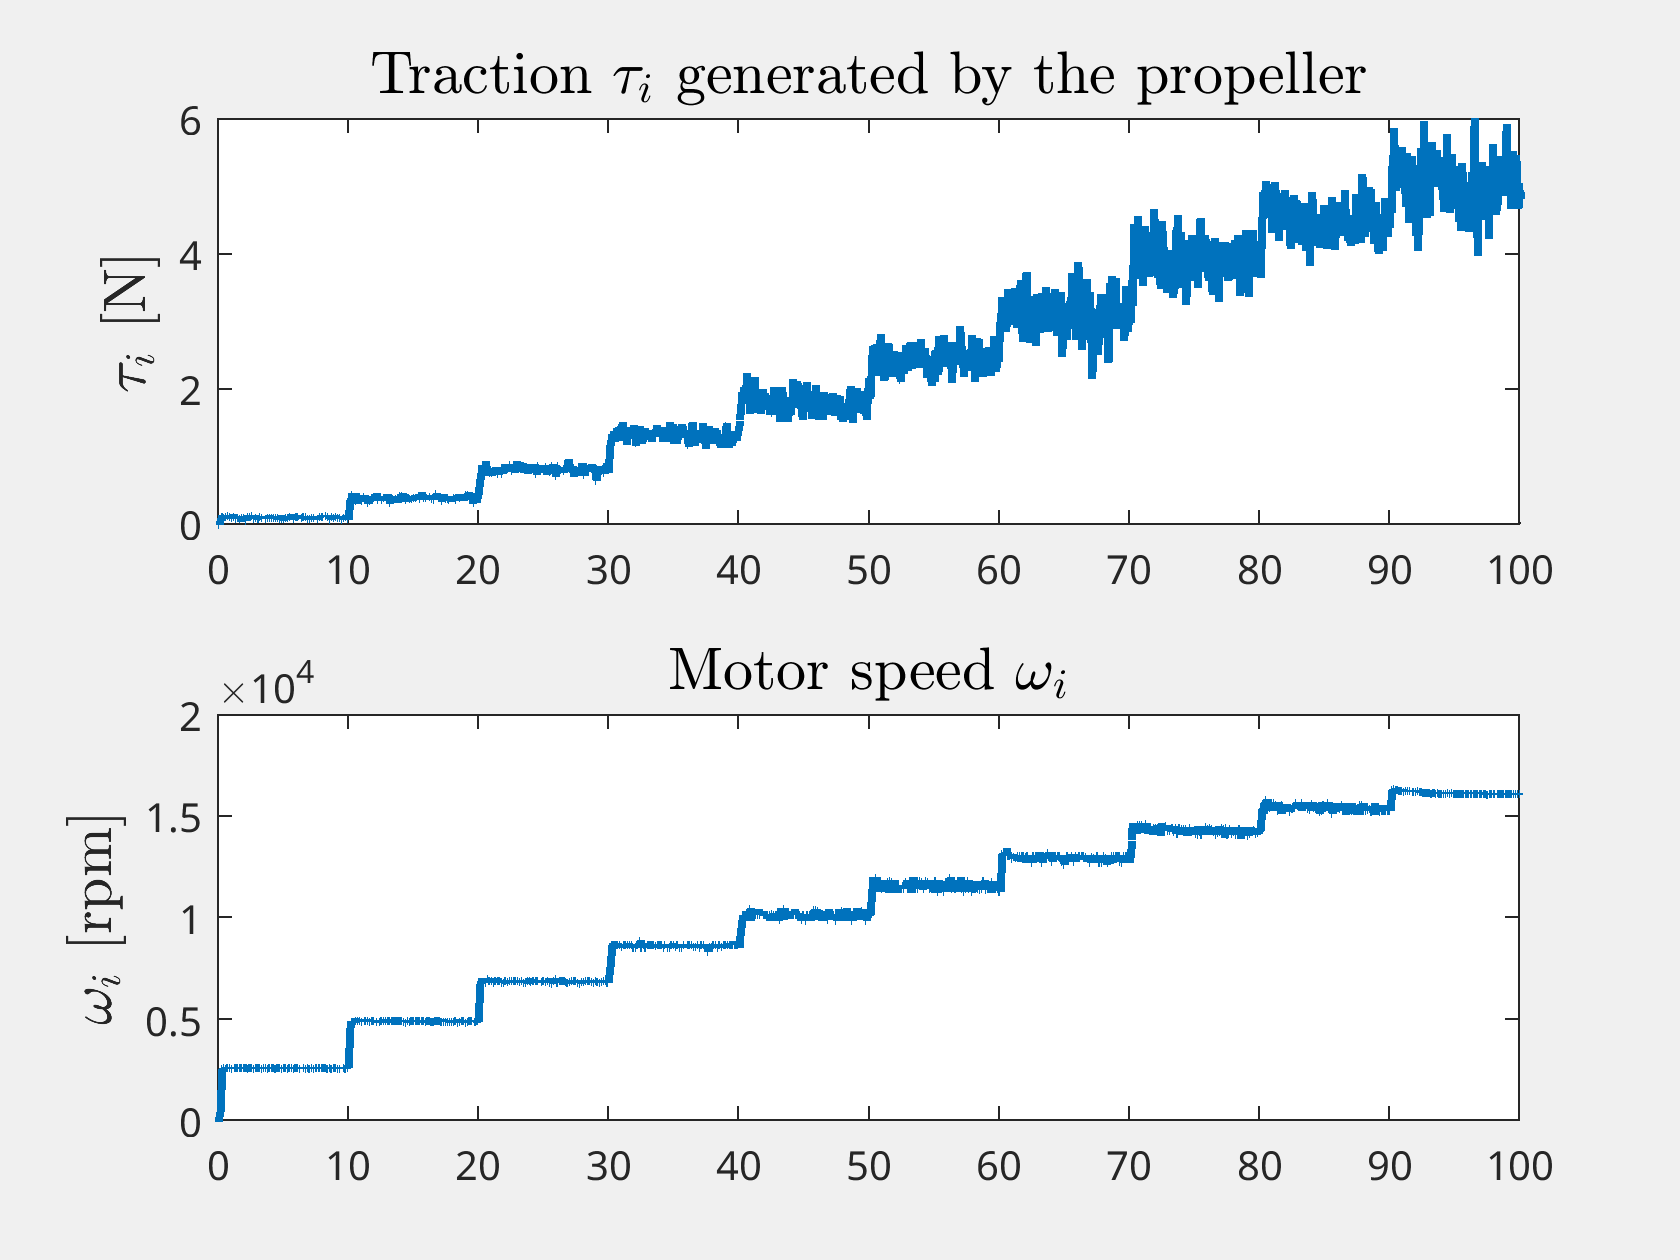
\includegraphics[trim=0cm 0cm 0cm 0cm,clip,width=1\columnwidth]{figures/ident_motor March 27 2024 1651.png}}
    \caption{Input-output response of an Esc-Motor-Propeller assembly.}
    \label{IOmot}
\end{figure}

\begin{figure}[ht!]
    \centerline{
    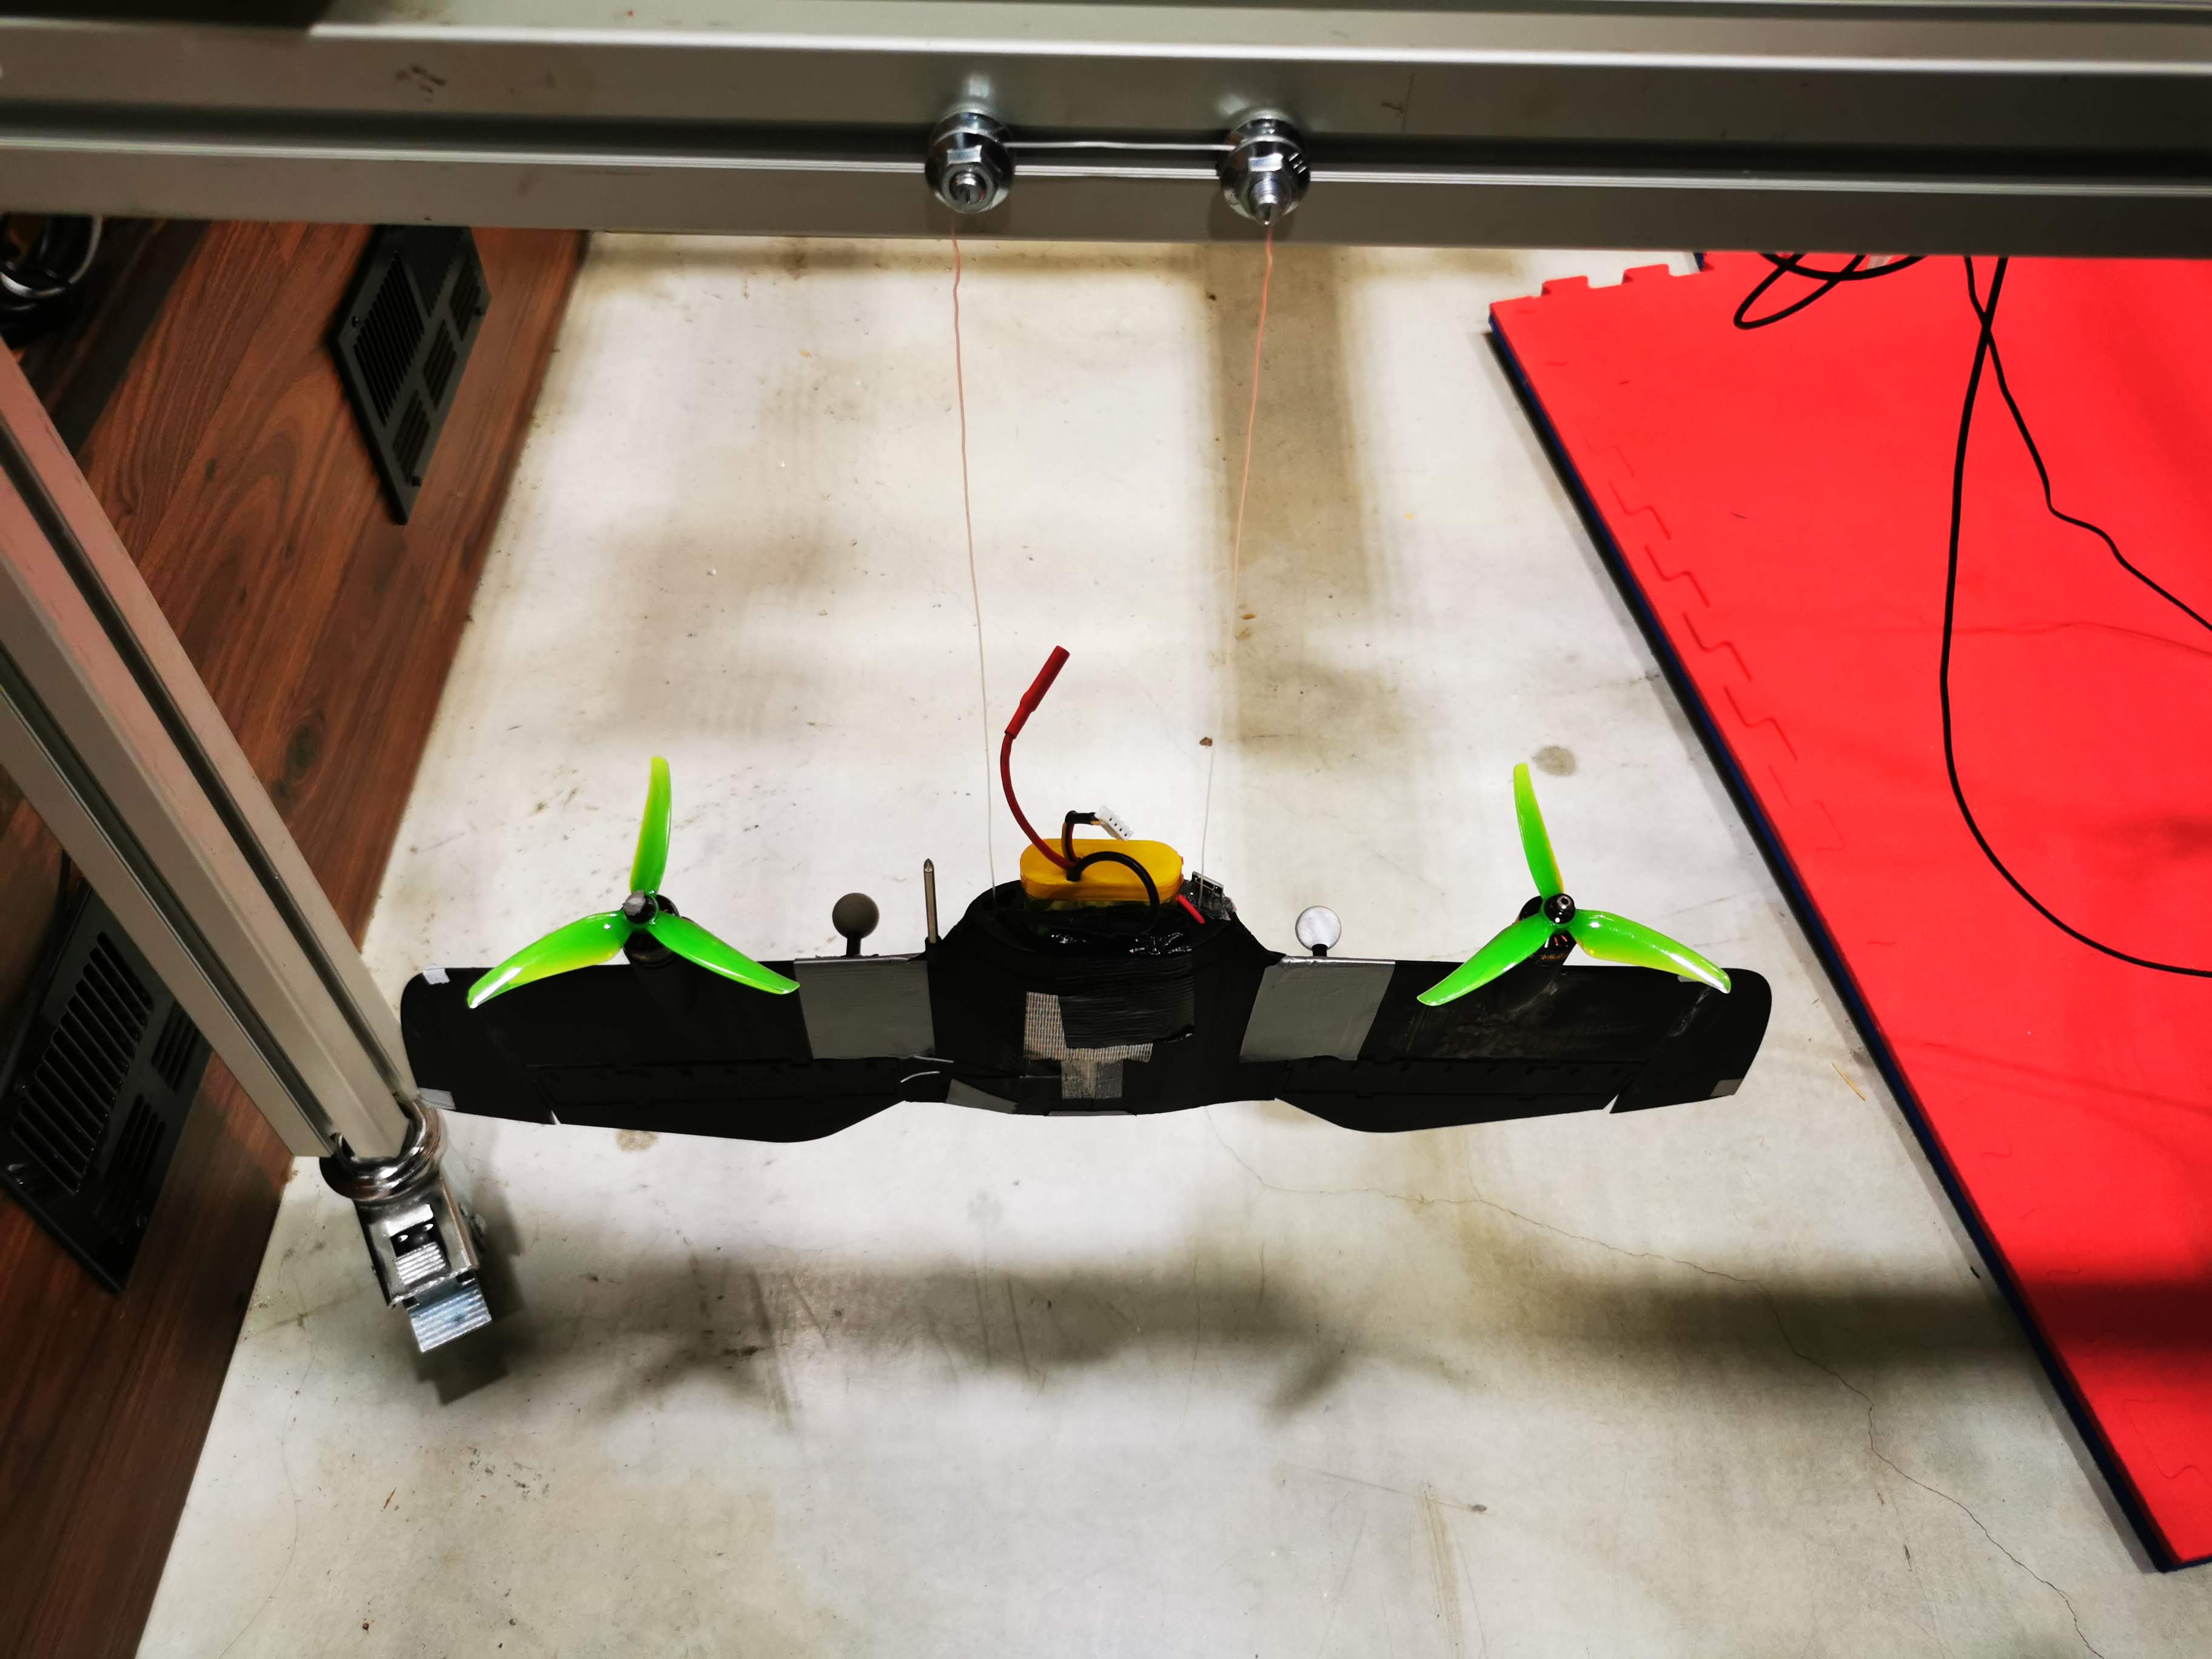
\includegraphics[trim=20cm 15cm 23cm 0cm,clip,width=0.6\columnwidth]{figures/IMG_20230609_085023.jpg}}
    \caption{Bifilar pendulum mounting for the identication of $\boldsymbol{J}$.}
    \label{fig:BifilarPend}
\end{figure}